%%%%%%%%%%%%%%%%%%%%%%%%%%%%%%%%%%%%%%%%%
% University/School Laboratory Report
% LaTeX Template
% Version 3.1 (25/3/14)
%
% This template has been downloaded from:
% http://www.LaTeXTemplates.com
%
% Original author:
% Linux and Unix Users Group at Virginia Tech Wiki 
% (https://vtluug.org/wiki/Example_LaTeX_chem_lab_report)
%
% License:
% CC BY-NC-SA 3.0 (http://creativecommons.org/licenses/by-nc-sa/3.0/)
%
%%%%%%%%%%%%%%%%%%%%%%%%%%%%%%%%%%%%%%%%%

%----------------------------------------------------------------------------------------
%	PACKAGES AND DOCUMENT CONFIGURATIONS
%----------------------------------------------------------------------------------------
\PassOptionsToPackage{table}{xcolor}

\documentclass[a4paper,twoside]{article}

\usepackage[a4paper,margin=1in]{geometry}
\usepackage[english]{babel}
\usepackage{fancyhdr}
\usepackage{titling}
\usepackage{lastpage}
\usepackage{subcaption}
\usepackage{graphicx}
\usepackage{enumitem}
\usepackage[toc,page]{appendix}

\usepackage[style=ieee, backend=biber]{biblatex}
\addbibresource{biblio.bib}

\usepackage{forloop}% http://ctan.org/pkg/forloop
\newcounter{loopcntr}
\newcommand{\rpt}[2][1]{%
	\forloop{loopcntr}{0}{\value{loopcntr}<#1}{#2}%
}

\usepackage[separate-uncertainty=true]{siunitx}
\DeclareSIUnit\sq{\ensuremath{\Box}}
\DeclareSIUnit\photon{ph}
\DeclareSIUnit\dec{dec}
\DeclareSIUnit\electron{e^-}
\DeclareSIUnit\LSB{LSB}
\DeclareSIUnit\rms{rms}
\sisetup{detect-weight=true,range-phrase = \text{--}}

\usepackage{hyperref}%
\usepackage{pdfpages}
\usepackage{booktabs}
\usepackage{multirow}
\usepackage{csvsimple}
\def\localpath{D:/Documents/PhD/FALCON/tex/data/}
\captionsetup[table]{position=bottom,skip=3pt}

\usepackage[siunitx, RPvoltages, arrowmos]{circuitikz}
\usepackage{tikz}
\usetikzlibrary{shapes,arrows,positioning,calc,automata}
\tikzset{
	font=\scriptsize,
	->, % makes the edges directed
	>=stealth, % makes the arrow heads bold
	node distance=3cm, % specifies the minimum distance between two nodes. Change if necessary.
	every state/.style={thick, fill=gray!10}, % sets the properties for each ’state’ node
	initial text=$ $, % sets the text that appears on the start arrow
}
% circuitikz
\ctikzset{tripoles/pmos style/nocircle}

\tikzstyle{mybox} = [draw=blue, fill=blue!20, very thick,
    rectangle, rounded corners, inner sep=0pt, inner ysep=5pt]

\usepackage{pgfplots}
\usetikzlibrary{pgfplots.groupplots}

\usepackage[nottoc]{tocbibind}


\usepackage[nottoc]{tocbibind}

\usepackage{amsmath, mathtools, amssymb}
\DeclareMathOperator*{\argmax}{arg\,max}
\DeclareMathOperator*{\argmin}{arg\,min}
\DeclareMathOperator\erf{erf}

\makeatletter
\newcommand*{\textoverline}[1]{$\overline{\hbox{#1}}\m@th$}
\makeatother

\usepackage{bytefield}
\usepackage[outline]{contour}
\contourlength{0.7pt}
\usepackage{afterpage}

%\usepackage{setspace}
%\onehalfspacing

\usepackage{url}
\renewcommand{\UrlFont}{\small}

%\setlength\parindent{0pt} % Removes all indentation from paragraphs

\renewcommand{\labelenumi}{\arabic{enumi}.} % Make numbering in the enumerate environment by number and not letter

% remove table of contents title
\makeatletter
\renewcommand\tableofcontents{%
	\@starttoc{toc}%
}
\makeatother

%\usepackage{times} % Uncomment to use the Times New Roman font

\pagestyle{fancy}
\fancyhf{}
\fancyhead[LE,RO]{pFREYA DAQ documentation}
\fancyhead[RE,LO]{\leftmark}
\fancyfoot[LE,RO]{P. Lazzaroni}
\fancyfoot[CE,CO]{Page \thepage\ of \pageref{LastPage}}
\fancyfoot[RE,LO]{\today}

\fancypagestyle{first}{%
	\fancyhf{}
	\renewcommand{\headrulewidth}{0pt}%
	\lfoot{P. Lazzaroni}
	\cfoot{Page \thepage\ of \pageref{LastPage}}
	\rfoot{\today}
}

%\usepackage{times} % Uncomment to use the Times New Roman font

%----------------------------------------------------------------------------------------
%	DOCUMENT INFORMATION
%----------------------------------------------------------------------------------------

\title{\fontsize{22}{18}\selectfont \textbf{pFREYA DAQ documentation}}
\author{\fontsize{16}{18}\selectfont Paolo \textsc{Lazzaroni}\\{\textmu}Lab\\Università degli Studi di Bergamo}

\begin{document}
	
	\maketitle\thispagestyle{empty} % Insert the title, author and date
	
	\section*{Summary}
	
	This document provides information on the Data AQuisition (DAQ) system to test the pFREYA16 and pFREYATS ASICs. The system is based on a Xilinx Ultrascale+ FPGA Evaluation Board (KCU116) and it is written in SystemVerilog/Verilog.
	
	\tableofcontents
	\clearpage
	
	\section{State machine}
	This section illustrates the state machine on the FPGA.
	\begin{figure}[h]
		\centering
		\scalebox{.65}{
			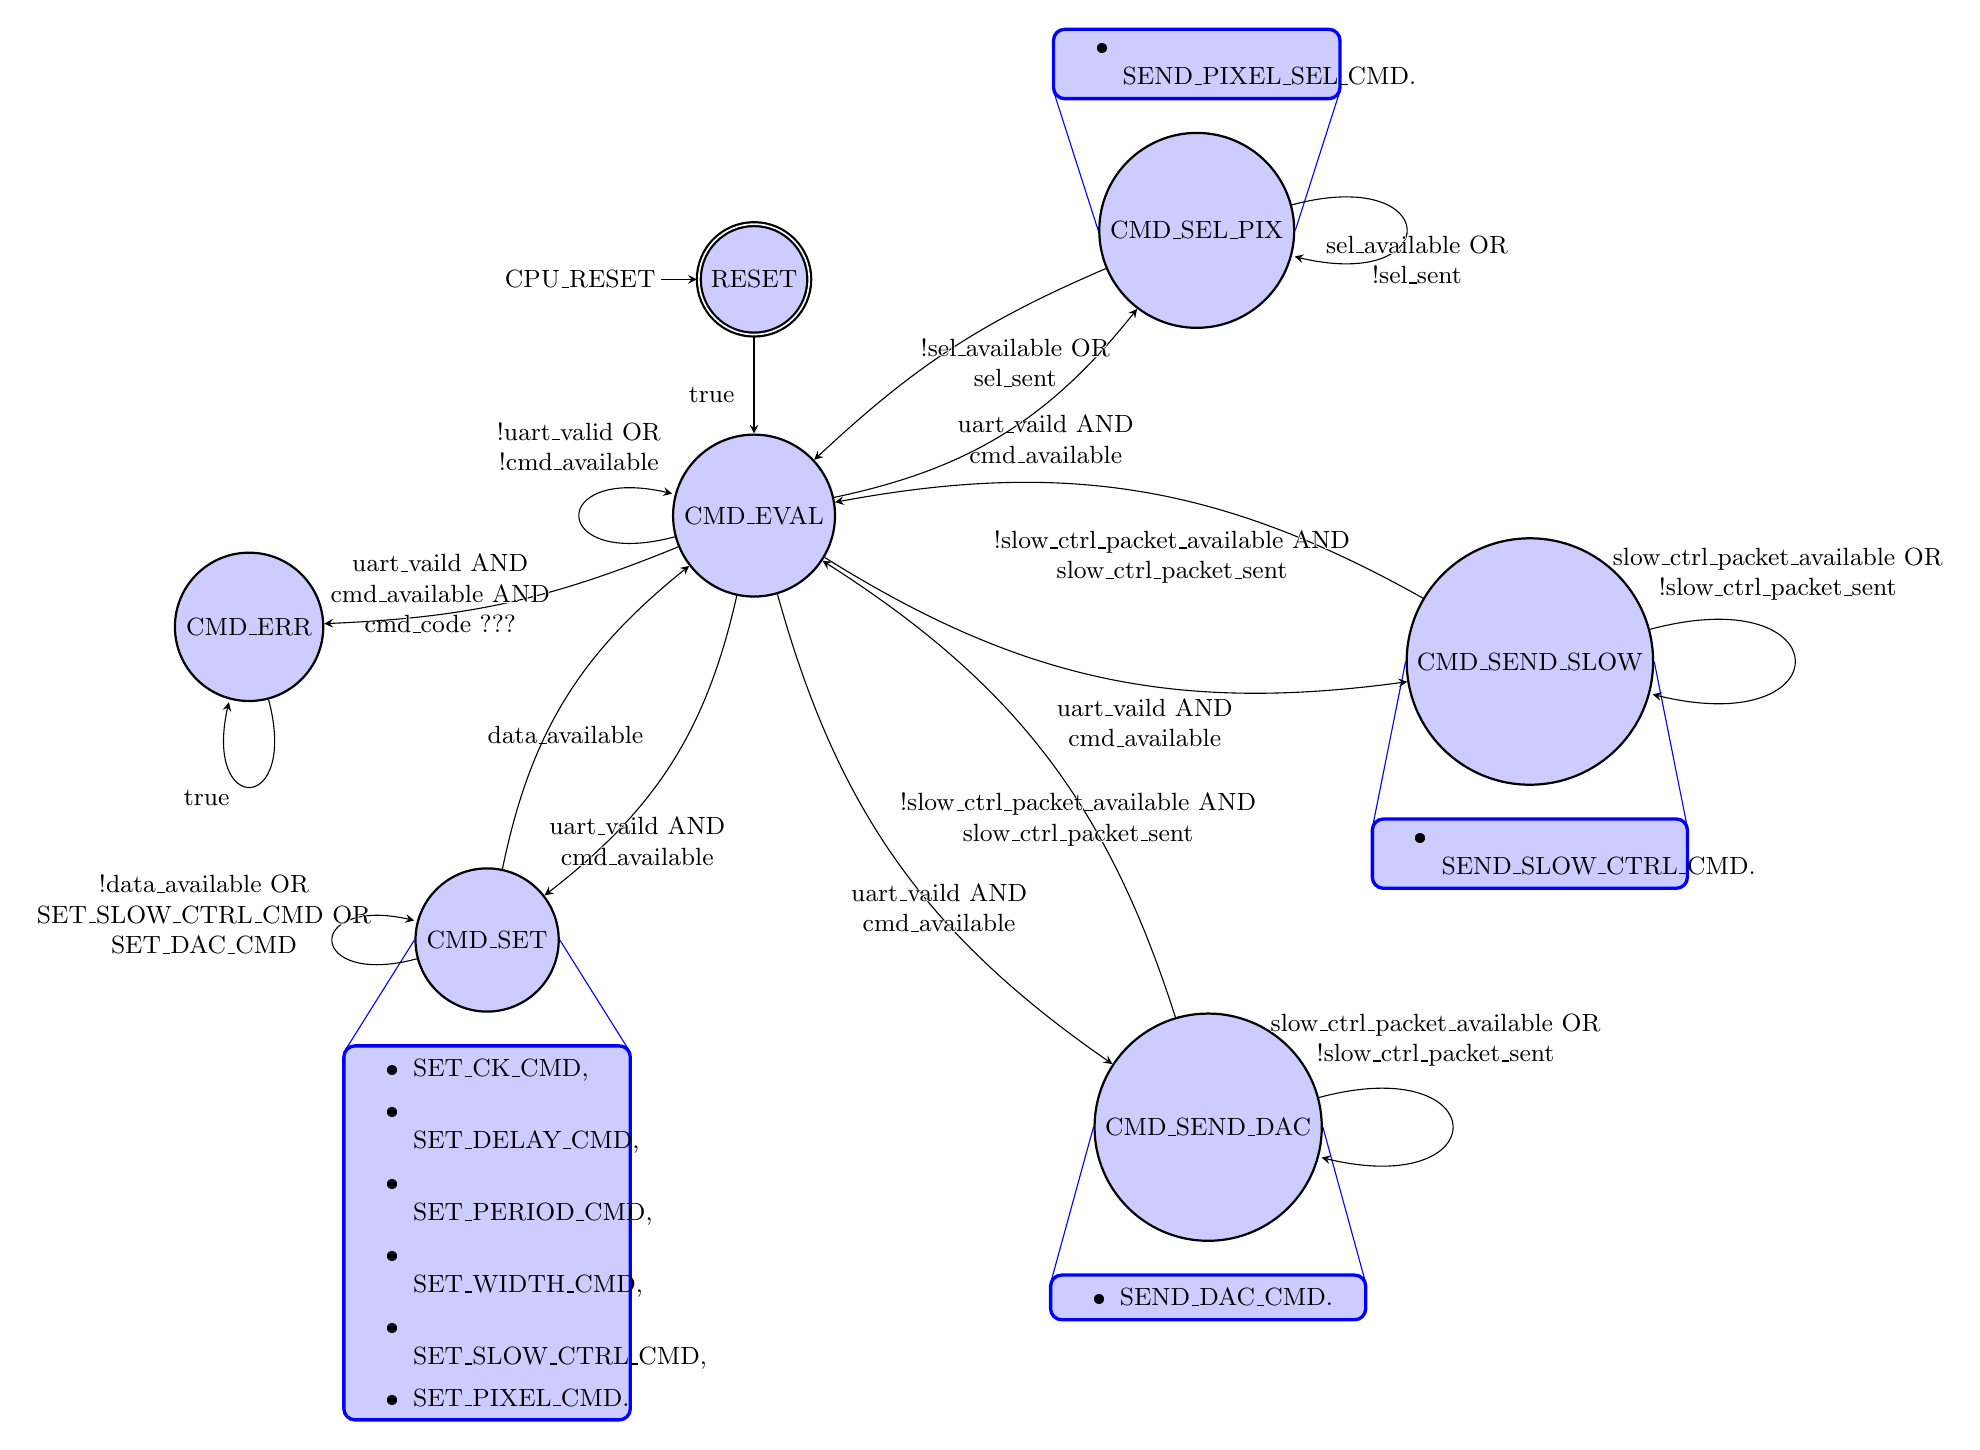
\begin{tikzpicture}
			\tikzstyle{every node}=[font=\small]
			\node[state, fill=blue!20, initial, accepting] (RESET) {RESET};
			\node[left=0.4cm of RESET] (CPU_RESET) {CPU\_RESET};
			\node[state, fill=blue!20, below of=RESET] (CMD_EVAL) {CMD\_EVAL};
			\node[state, fill=blue!20, below left=0cm and 5cm of CMD_EVAL] (CMD_ERR) {CMD\_ERR};
			\node[state, fill=blue!20, below left=4cm and 2cm of CMD_EVAL, align=center] (CMD_SET) {CMD\_SET};
			\node[state, fill=blue!20, below right=6cm and 4cm of CMD_EVAL, align=center] (CMD_SEND_DAC) {CMD\_SEND\_DAC};
			\node[state, fill=blue!20, below right=0cm and 8cm of CMD_EVAL, align=center] (CMD_SEND_SLOW) {CMD\_SEND\_SLOW};
			\node[state, fill=blue!20, above right=2cm and 4cm of CMD_EVAL, align=center] (CMD_SEL_PIX) {CMD\_SEL\_PIX};
			
			\node[mybox, below=0.4cm of CMD_SET] (SET_BOX) {%
				\begin{minipage}[t!]{0.3\textwidth}
					\begin{itemize}
						\item SET\_CK\_CMD,
						\item SET\_DELAY\_CMD,
						\item SET\_PERIOD\_CMD,
						\item SET\_WIDTH\_CMD,
						\item SET\_SLOW\_CTRL\_CMD,
						\item SET\_PIXEL\_CMD.
					\end{itemize}
				\end{minipage}
				};
			\draw[blue,-] ($(SET_BOX.north west) + (0.03,-0.09)$) -- (CMD_SET.west);
			\draw[blue,-] ($(SET_BOX.north east) + (-0.03,-0.09)$) -- (CMD_SET.east);
			\node[mybox, below=0.4cm of CMD_SEND_SLOW] (CMD_SEND_SLOW_BOX) {%
				\begin{minipage}[t!]{0.33\textwidth}
					\begin{itemize}
						\item SEND\_SLOW\_CTRL\_CMD.
					\end{itemize}
				\end{minipage}
				};
			\draw[blue,-] ($(CMD_SEND_SLOW_BOX.north west) + (0.03,-0.09)$) -- (CMD_SEND_SLOW.west);
			\draw[blue,-] ($(CMD_SEND_SLOW_BOX.north east) + (-0.03,-0.09)$) -- (CMD_SEND_SLOW.east);
			\node[mybox, above=0.4cm of CMD_SEL_PIX] (CMD_SEL_PIX_BOX) {%
				\begin{minipage}[t!]{0.3\textwidth}
					\begin{itemize}
						\item SEND\_PIXEL\_SEL\_CMD.
					\end{itemize}
				\end{minipage}
				};
			\draw[blue,-] ($(CMD_SEL_PIX_BOX.south west) + (0.03,0.09)$) -- (CMD_SEL_PIX.west);
			\draw[blue,-] ($(CMD_SEL_PIX_BOX.south east) + (-0.03,0.09)$) -- (CMD_SEL_PIX.east);
			\node[mybox, below=0.4cm of CMD_SEND_DAC] (CMD_SEND_DAC_BOX) {%
				\begin{minipage}[t!]{0.33\textwidth}
					\begin{itemize}
						\item SEND\_DAC\_CMD.
					\end{itemize}
				\end{minipage}
				};
			\draw[blue,-] ($(CMD_SEND_DAC_BOX.north west) + (0.03,-0.09)$) -- (CMD_SEND_DAC.west);
			\draw[blue,-] ($(CMD_SEND_DAC_BOX.north east) + (-0.03,-0.09)$) -- (CMD_SEND_DAC.east);

			\draw (RESET) edge[below] node[label=left:true]{} (CMD_EVAL);
			\draw (CMD_EVAL) edge[below, bend left=20] node[below left=1.4cm and 0.3cm, label={[align=center]\contour{white}{uart\_vaild AND}\\\contour{white}{cmd\_available}}]{} (CMD_SET);
			\draw (CMD_EVAL) edge[loop left] node[above=0.2cm, label={[align=center]!uart\_valid OR\\!cmd\_available}]{} (CMD_EVAL);
			\draw (CMD_EVAL) edge[below, bend left=10] node[below left=0.5cm and 0.7cm, label={[align=center]\contour{white}{uart\_vaild AND}\\\contour{white}{cmd\_available AND}\\\contour{white}{cmd\_code ???}}]{} (CMD_ERR);
			\draw (CMD_ERR) edge[loop below] node[label=left:true]{} (CMD_ERR);
			\draw (CMD_SET) edge[loop left] node[below left=0.3cm and 1.5cm, label={[align=center]\contour{white}{!data\_available OR}\\\contour{white}{SET\_SLOW\_CTRL\_CMD OR}\\\contour{white}{SET\_DAC\_CMD}}]{} (CMD_SET);
			\draw (CMD_SET) edge[below, bend left=20] node[below=0.7cm, label=\contour{white}{data\_available}]{} (CMD_EVAL);
			\draw (CMD_EVAL) edge[below, bend right=20] node[below right=1.0cm and 0.4cm, label={[align=center]\contour{white}{uart\_vaild AND}\\\contour{white}{cmd\_available}}]{} (CMD_SEND_DAC);
			\draw (CMD_SEND_DAC) edge[right, bend right=20] node[below right=1.3cm and 0.3cm, label={[align=center]\contour{white}{!slow\_ctrl\_packet\_available AND}\\\contour{white}{slow\_ctrl\_packet\_sent}}]{} (CMD_EVAL);
			\draw (CMD_SEND_DAC) edge[loop right] node[above left=0.4cm and 0.1cm, label={[align=center]\contour{white}{slow\_ctrl\_packet\_available OR}\\\contour{white}{!slow\_ctrl\_packet\_sent}}]{} (CMD_SEND_DAC);
			\draw (CMD_EVAL) edge[below, bend right=20] node[below right=1.0cm and 0.4cm, label={[align=center]\contour{white}{uart\_vaild AND}\\\contour{white}{cmd\_available}}]{} (CMD_SEND_SLOW);
			\draw (CMD_SEND_SLOW) edge[right, bend right=20] node[below right=1.3cm and 0.3cm, label={[align=center]\contour{white}{!slow\_ctrl\_packet\_available AND}\\\contour{white}{slow\_ctrl\_packet\_sent}}]{} (CMD_EVAL);
			\draw (CMD_SEND_SLOW) edge[loop right] node[above left=0.4cm and 0.1cm, label={[align=center]\contour{white}{slow\_ctrl\_packet\_available OR}\\\contour{white}{!slow\_ctrl\_packet\_sent}}]{} (CMD_SEND_SLOW);
			\draw (CMD_EVAL) edge[below, bend right=20] node[below right=0.5cm and 0.4cm, label={[align=center]\contour{white}{uart\_vaild AND}\\\contour{white}{cmd\_available}}]{} (CMD_SEL_PIX);
			\draw (CMD_SEL_PIX) edge[right, bend right=10] node[below right=0.6cm and 0.7cm, label={[align=center]\contour{white}{!sel\_available OR}\\\contour{white}{sel\_sent}}]{} (CMD_EVAL);
			\draw (CMD_SEL_PIX) edge[loop right] node[below right=0.8cm and 0cm, label={[align=center]\contour{white}{sel\_available OR}\\\contour{white}{!sel\_sent}}]{} (CMD_SEL_PIX);
		\end{tikzpicture}
		}
	\end{figure}

	\section{General directions}
	The state machine might seem messy, but the fact is that it is just hard to render with that instrument the way the FPGA works. So a few words of clarification. When saying first, second, ... it is intended as ``starting from the MSB''.

	When the FPGA is turned up it should be in RESET state. If a layer of assurance is needed one can push the CPU\_RESET button on the FPGA.

	Right after the reset is released, the FPGA goes in the CMD\_EVAL state, waiting for UART communication. It stays there until a UART communication is available. If the communication is not one of those envisioned, it goes in the CMD\_ERR state and stays there forever (or until the CPU\_RESET button is pressed).

	The UART communication is an 8-bit packet that comes in two flavours: command and data packet. A command to be sent in the UART is composed of an initial 0, to identify a command packet, followed by four bits identifying the command and three bits identifying the signal the command is referring to, if any. A data packet is instead introduced by a 1, followed by 7 bits representing the data content. Please refer to \texttt{pFREYA\_defs.sv} for which bit sequence corresponds to which command/data.

	If the command is one between SET\_CK\_CMD, SET\_DELAY\_CMD, SET\_HIGH\_CMD, SET\_LOW\_CMD, SET\_SLOW\_CTRL\_CMD, SET\_DAC\_CMD, and SET\_PIXEL\_CMD, the FPGA goes in the CMD\_SET state. In this state the command and the signal are checked:
	\begin{itemize}
		\item SET\_CK\_CMD sets a clock, so a signal with 50\% duty cycle, and the three following bits represent a clock signal (SLOW\_CTRL\_CK\_CODE, SEL\_CK\_CODE, ADC\_CK\_CODE, INJ\_STB\_CODE, SER\_CK\_CODE, DAC\_SCK\_CODE) to be set.
		\item SET\_DELAY\_CMD, SET\_HIGH\_CMD, and SET\_LOW\_CMD set a fast signal characteristic, that are delay and how long will it stay high or low. The three following bits represent a fast control signal (CSA\_RESET\_N\_CODE, SH\_INF\_CODE, SH\_SUP\_CODE, ADC\_START\_CODE, and INJ\_START which is not used right now).
	\end{itemize}

	After one of these commands, the FPGA expect a data packet transmission, representing a time length expressed in FPGA clocks. The FPGA clock is a 200 MHz clock generated by the SYSTEM CLOCKs (P and N) running at 300 MHz through a clock wizard instance. However, since each event is triggered on the rising edge of the base clock, the fastest signal attainable has a frequency of 100 MHz (200 MHz divided by 2, which is triggering just on the rising edge).

	The data packet expected are composed of 7-bit binary data representing the number of FPGA clocks that the signal property (period, delay, high, or low) has to be set to. Be mindful that the clocks are set by period, while fast signal are set by high and low, which is different. The data packet received set the proper divider with which the counter for each property is checked in order to commute the state of the wanted signal.

	The commands SET\_SLOW\_CTRL\_CMD and SET\_DAC\_CMD still end up in the CMD\_SET state, but need more than a 7-bit data to work with. Specifically for the SET\_SLOW\_CTRL\_CMD a 122-bit data is needed (rounded up to 128-bit in FPGA registers, where the MSB are not interesting), while for SET\_DAC\_CMD a 24-bit data is needed (rounded up to 32-bit in FPGA registers, where the MSB are not interesting). Both the sub-state expect a different kind of data packet: the first bit identifies again the data packet, and it is set to 1, while the second bit is either 1 or 0, if this is the last packet or not respectively. The effective number of bits available for data is therefore 6. The SET\_SLOW\_CTRL\_CMD expect 19 data packets, while SET\_DAC\_CMD needs 4 of them. Be mindful of setting the right second bit for each packet. The data are stored in FPGA registers and once ready can be sent through the proper command. Please refer to the ASIC documentation of the DAC documentation for the meaning of each bit. A summary is also done in the \texttt{pFREYA\_defs.sv} file.

	The command SET\_PIXEL\_CMD is yet another exception. It needs a signal, representing either row or column of the pixel to be readout. The data packet is the same as those in the clocks or fast controls, but represents the number of the pixel to be selected. The selection is then sent through the proper command.

	The commands SEND\_SLOW\_CTRL\_CMD and SEND\_DAC\_CMD are used to forward the content of the respective register to the ASIC and the DAC on the pFREYA mother board. They both work in the same way, meaning like a SPI communication. Basically the bits are sent in a serial way, with a clock together with them to provide the time basis on the shift registers in the ASIC or the DAC. A signal enabling the communication is also provided.

	Finally, the command SEND\_PIXEL\_SEL\_CMD sends the pixel selection to the ASIC, based on the pixel row and col set. The pixel selection is done by moving a high state in a shift register, therefore a number of clock equal to the pixel row or col to be selected is generated by the FPGA, together with the signal enabling the communication.
%----------------------------------------------------------------------------------------
%	BIBLIOGRAPHY
%----------------------------------------------------------------------------------------

\clearpage
\nocite{*}
\printbibliography
%----------------------------------------------------------------------------------------


\end{document}